\chapter{对其他组项目的交叉测试报告}
\section{测试对象、材料来源与范围}
本章收录项目组提供的《第十组交叉测试报告》，测试对象为其他组的 test10 项目，不是本组轻量级外卖服务平台。附件原报告日期为 2026 年 9 月 17 日，截图文件记录日期为 9 月 16 日。验收依据为被测项目的 \code{docs/SRS.md}；其需求范围、账号模型和订单状态与本组 SRS 不同，不能直接套用本组标准评价对方。

附件没有提供被测项目的仓库地址、提交号和运行环境版本，因此本章保留 test10 标识及原有验收口径，不补写无法核实的版本信息。以下原报告中的“本轮”均指附件所记录的那轮测试；此次整理没有重新运行对方系统。原始 LaTeX、配置和全部截图另行原样附在源码包中，正文仅调整标题层级及图片相对路径以接入本报告。

本轮主要发现与后续建议集中在超库存输入缺少明确反馈、订单快照需变更后反向验证、库存扣减与取消恢复需数据库证据、越权接口与事务回滚需补测等方面。报告未将“未测试”直接判为缺陷，也未把对方 SRS 明确排除的支付、骑手配送或地址簿当作缺失功能。
\section{验收方法与判定口径}\label{1-ux9a8cux6536ux65b9ux6cd5ux4e0eux5224ux5b9aux53e3ux5f84}

本报告严格按照 \texttt{docs/SRS.md}
的需求编号进行验收，不把``真实外卖平台通常应该有''的功能擅自加入判定范围。每一个需求条目主要通过真实页面操作进行比对，必要时结合页面提示和已有接口现象判断，并将结果区分为：

\begin{itemize}
\tightlist
\item
  \textbf{已实现并通过}：本轮通过真实页面操作获得了明确结果和截图证据
\item
  \textbf{部分实现或证据不足}：主流程可以运行，但仍缺少边界、接口、事务或数据层证据
\item
  \textbf{本轮未测试}：本轮没有安排或没有条件覆盖，不直接判定为未实现
\item
  \textbf{不属于当前范围}：SRS 已明确不要求，本轮不作为缺陷处理
\end{itemize}

本轮使用的测试账号为用户 A（13800000001）、用户
B（13800000002）和商家用户
C（13800000003），测试店铺为``验收餐厅X''和``验收餐厅Y''，商品为``验收牛肉饭''和``验收奶茶''。所有截图均来自本地真实运行页面，图片已嵌入对应需求条目下。

\section{用户模块需求对照}\label{2-ux7528ux6237ux6a21ux5757ux9700ux6c42ux5bf9ux7167}

\subsection{FR-USER-01
用户注册}\label{fr-user-01-ux7528ux6237ux6ce8ux518c}

\textbf{需求目标}：使用手机号、密码和验证码注册 User，同时原子创建
Account 与 User，注册成功后不自动登录、不返回 Token，密码不得明文保存

\textbf{实际验收}：使用三个测试手机号分别完成注册，注册成功后跳转登录页，随后使用用户
A 登录成功。重复注册用户 A
的手机号时，页面提示``手机号已被注册''，说明手机号唯一性和重复注册拦截已生效

\pandocbounded{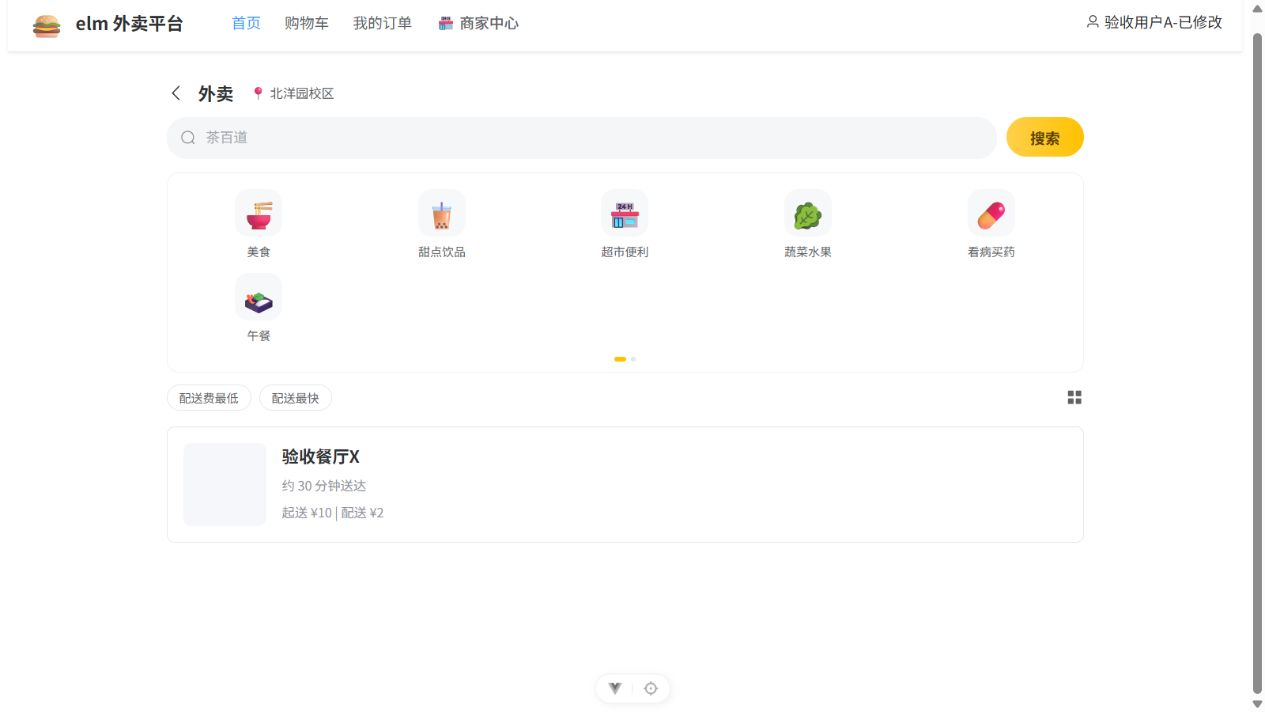
\includegraphics[keepaspectratio,alt={用户注册及首页证据}]{figures/cross/2026-9-16-sep-elm-SRS验收截图-01-用户首页.png}}

\textbf{已实现部分}：正常注册、重复手机号拦截、注册成功不自动登录，用户能够用新账号重新登录

\textbf{本轮未测试项}：手机号全部格式、验证码错误和过期、注册失败后的数据回滚、密码存储方式等边界，本轮主要确认正常注册和重复手机号场景

\textbf{改进建议}：补充手机号和验证码的完整边界测试，并用接口响应和数据库查询确认失败注册不会留下孤立
Account、User 或错误验证码状态

\subsection{FR-USER-02
获取注册验证码}\label{fr-user-02-ux83b7ux53d6ux6ce8ux518cux9a8cux8bc1ux7801}

\textbf{需求目标}：服务端生成 6
位数字验证码，并绑定手机号、保存有效期，演示模式可以通过响应返回验证码，非演示模式不得泄露给前端

\textbf{实际验收}：注册流程中使用了演示环境验证码，页面能够获取并使用验证码完成注册，说明当前演示开关和联调路径可用

\textbf{已实现部分}：演示验证码可以支撑本地注册流程，服务能够返回可用于联调的验证码

\textbf{本轮未测试项}：验证码过期、错误验证码、不同手机号之间的验证码隔离和非演示环境返回值，本轮主要确认演示模式能够支撑真实注册

\textbf{改进建议}：分别使用两个手机号交叉填写验证码，测试过期和错误验证码，并保留接口响应截图，确认验证码不会跨手机号复用

\subsection{FR-USER-03
用户登录}\label{fr-user-03-ux7528ux6237ux767bux5f55}

\textbf{需求目标}：统一 Account
使用手机号和密码登录，手机号不存在与密码错误统一返回 401，DISABLED
账号不得登录，成功后返回 Account 级 Token，Token TTL 为 7 天

\textbf{实际验收}：用户 A
使用正确密码登录后进入首页并显示昵称和店铺；使用错误密码时页面统一提示``手机号或密码错误''

\pandocbounded{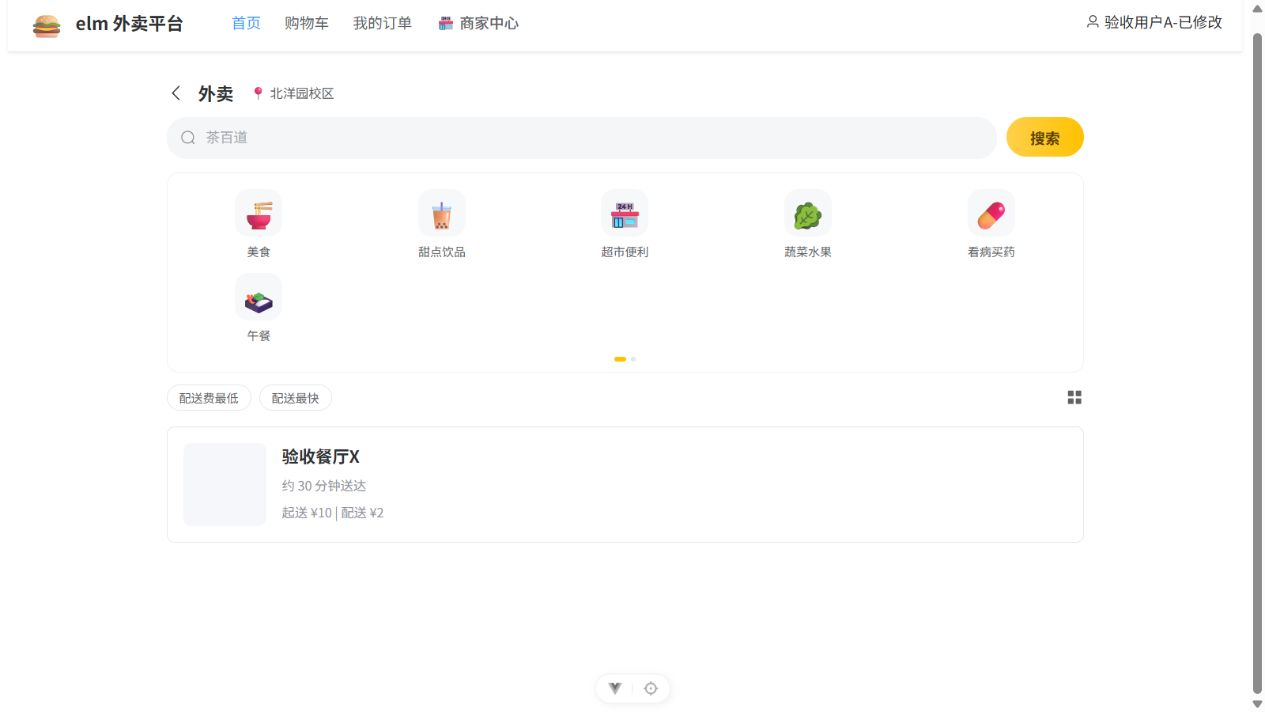
\includegraphics[keepaspectratio,alt={登录成功证据}]{figures/cross/2026-9-16-sep-elm-SRS验收截图-01-用户首页.png}}

\pandocbounded{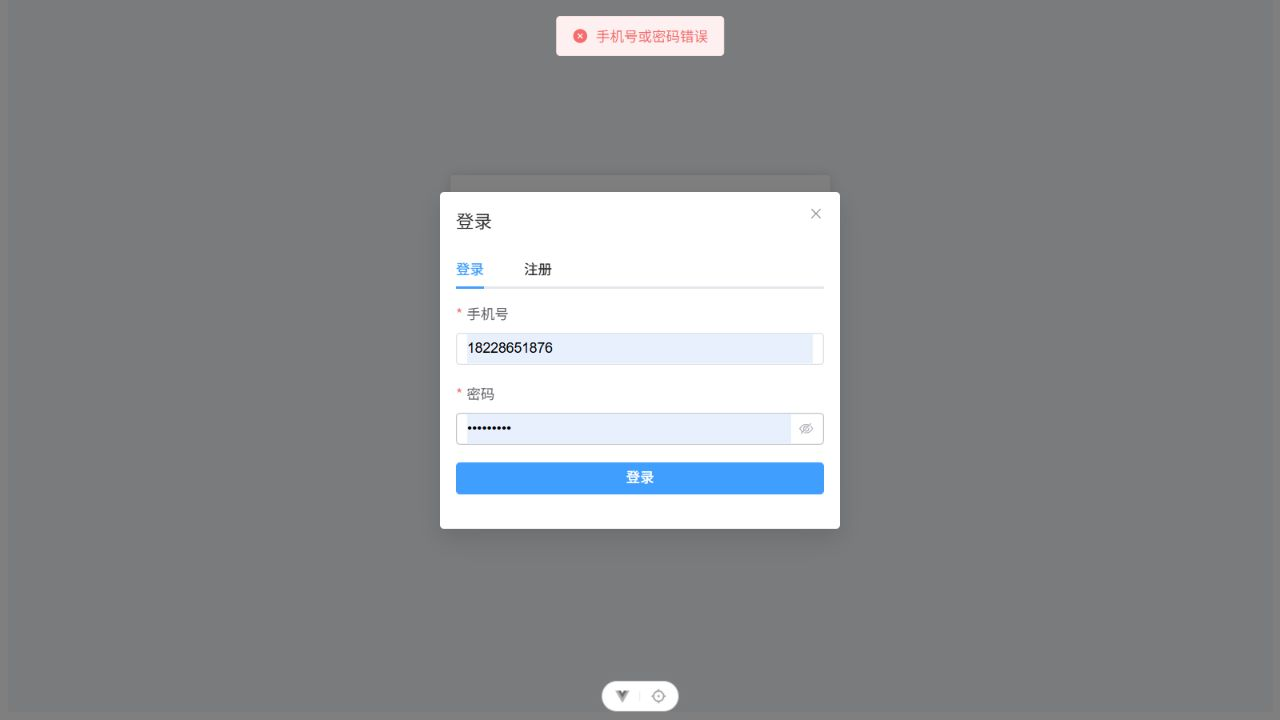
\includegraphics[keepaspectratio,alt={错误密码证据}]{figures/cross/2026-9-16-sep-elm-SRS验收截图-错误密码登录.png}}

\textbf{已实现部分}：手机号密码登录、统一错误提示、登录后进入用户首页、Token
驱动的认证访问

\textbf{本轮未测试项}：禁用账号、过期登录状态和无登录状态直达页面，本轮主要确认正常登录和错误密码提示符合需求

\textbf{改进建议}：增加禁用账号登录用例、过期 Token 用例和无 Token
访问用例，确认页面提示与 SRS 规定的 401/403 语义一致

\subsection{FR-USER-04
查询个人信息}\label{fr-user-04-ux67e5ux8be2ux4e2aux4ebaux4fe1ux606f}

\textbf{需求目标}：已登录用户查询自己的 User.id、手机号、昵称和账号状态

\textbf{实际验收}：用户 A
进入个人信息页面，手机号以只读方式显示，昵称和账号信息能够正常展示

\pandocbounded{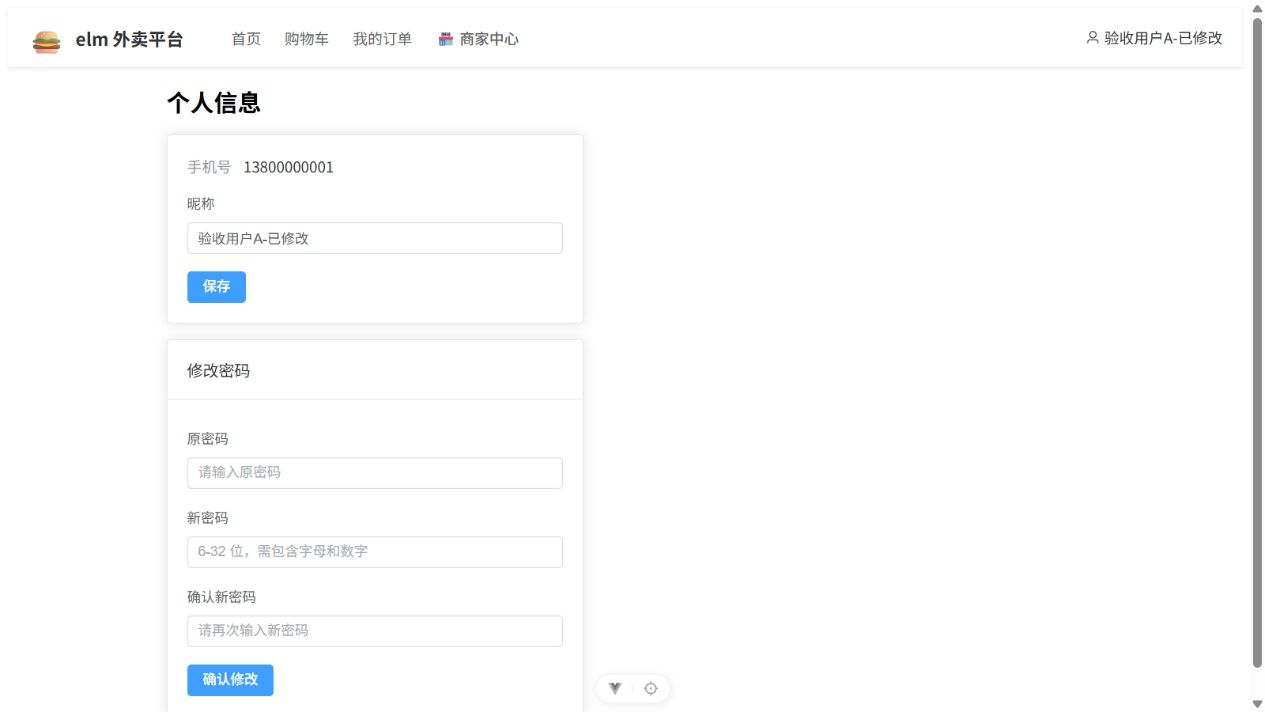
\includegraphics[keepaspectratio,alt={个人资料证据}]{figures/cross/2026-9-16-sep-elm-SRS验收截图-个人资料持久化.png}}

\pandocbounded{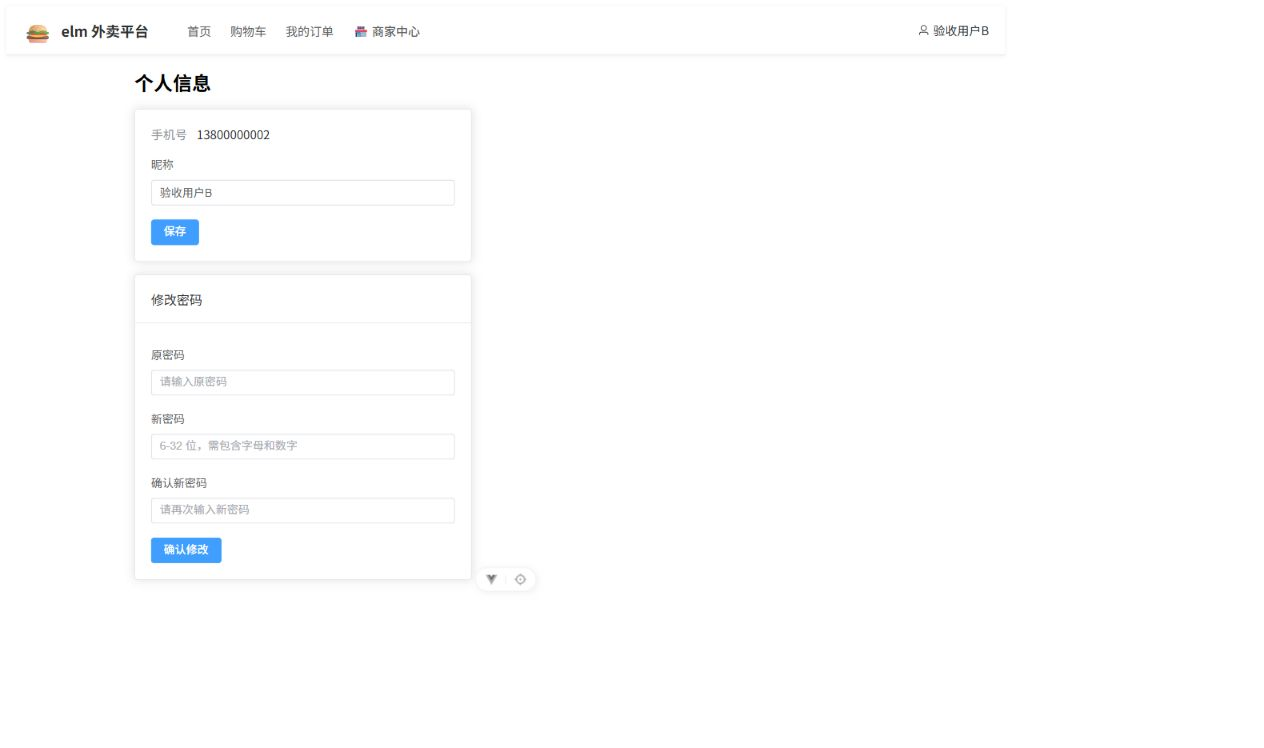
\includegraphics[keepaspectratio,alt={补充的个人资料页面}]{figures/cross/2026-9-16-sep-elm-SRS对照验收-个人资料页面.png}}

\textbf{结论}：已实现并通过页面验证，跨用户数据隔离还需要配合越权接口测试进一步确认

\subsection{FR-USER-05
修改个人信息}\label{fr-user-05-ux4feeux6539ux4e2aux4ebaux4fe1ux606f}

\textbf{需求目标}：只能修改自己的 nickname，不得通过该接口修改
phone、password、account.id 或 account.status

\textbf{实际验收}：用户 A
修改昵称为``验收用户A-已修改''，刷新页面后仍保持新昵称，手机号仍为只读状态

\textbf{结论}：已实现并通过。当前未发现可以从个人资料页面修改手机号或密码的入口

\textbf{改进建议}：通过接口直接提交 phone、password、account.status
等额外字段，确认后端不会接受未定义字段或发生越权修改

\subsection{FR-USER-06
修改密码}\label{fr-user-06-ux4feeux6539ux5bc6ux7801}

\textbf{需求目标}：已登录用户使用 oldPassword 和 newPassword
修改密码，新密码沿用注册规则，错误原密码返回``原密码错误''，已有 Token
按 SRS 继续生效

\textbf{实际验收}：用户 A
修改密码成功后使用新密码登录，旧密码登录失败；输入``abc''时提示密码必须为
6-32 位且同时包含字母和数字；错误原密码被拒绝

\pandocbounded{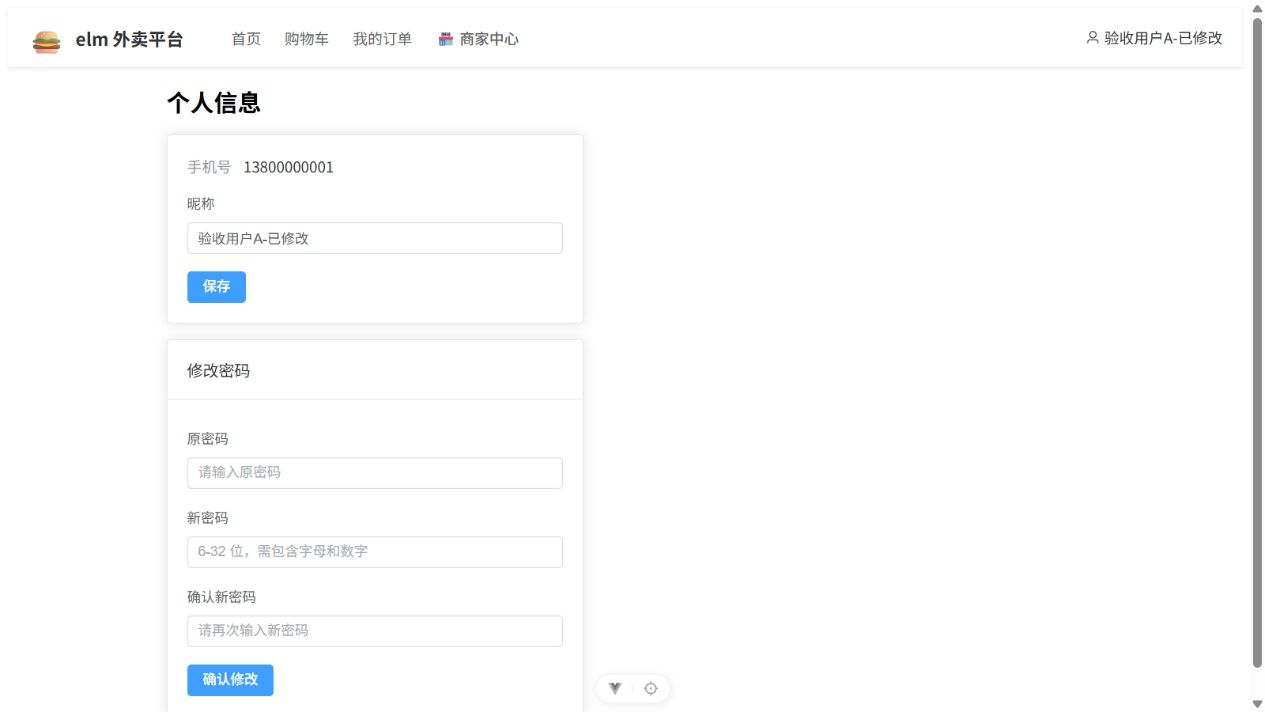
\includegraphics[keepaspectratio,alt={修改密码证据}]{figures/cross/2026-9-16-sep-elm-SRS验收截图-修改密码.png}}

\pandocbounded{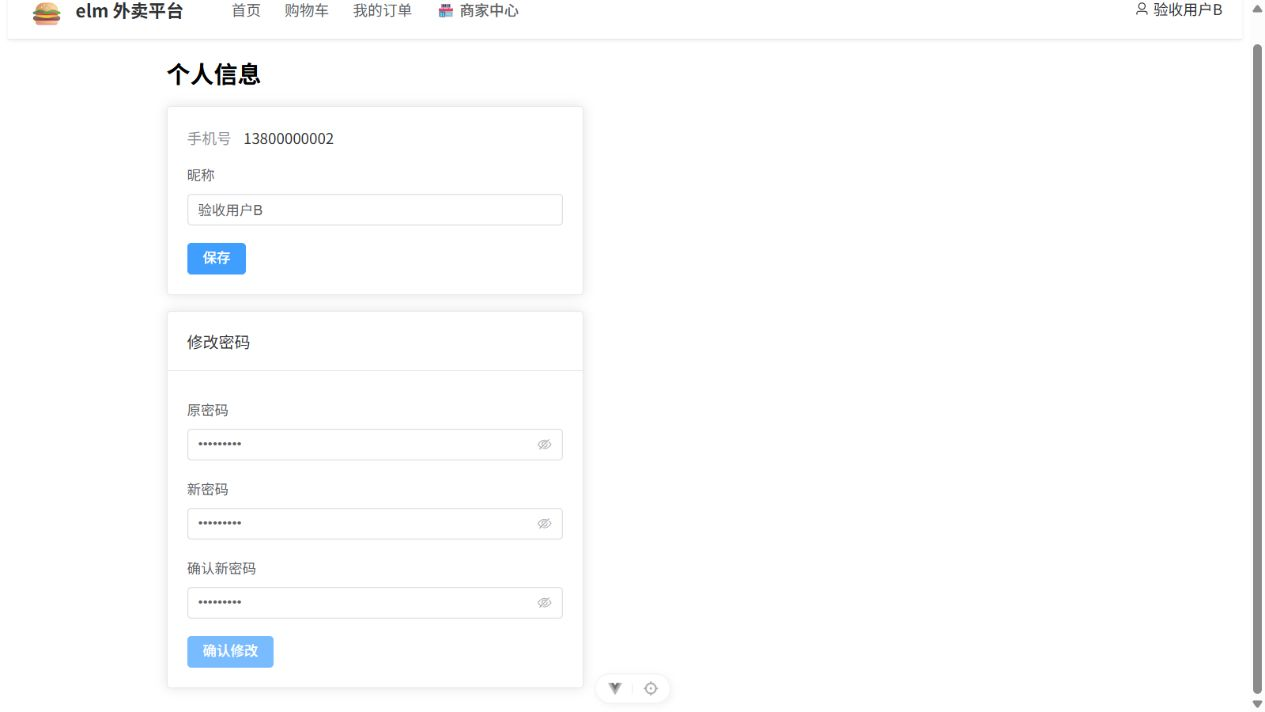
\includegraphics[keepaspectratio,alt={密码边界证据}]{figures/cross/2026-9-16-sep-elm-SRS验收截图-密码边界.png}}

\textbf{结论}：核心功能和已测边界通过

\textbf{本轮未测试项}：修改密码后的旧 Token
状态、长度上限、相同新旧密码和空白处理，本轮主要确认正确密码、错误原密码和非法新密码均有反馈

\section{商家、店铺和商品需求对照}\label{3-ux5546ux5bb6ux5e97ux94faux548cux5546ux54c1ux9700ux6c42ux5bf9ux7167}

\subsection{FR-MERCHANT-01
商家注册与身份开通}\label{fr-merchant-01-ux5546ux5bb6ux6ce8ux518cux4e0eux8eabux4efdux5f00ux901a}

\textbf{需求目标}：在已有 Account 上追加一个
Merchant，不创建第二套登录账号，不删除 User 身份，一个 Account
最多关联一个 Merchant

\textbf{实际验收}：用户 C 注册并登录后开通 Merchant 身份，仍可保留普通
User 身份，并进入商家工作台

\pandocbounded{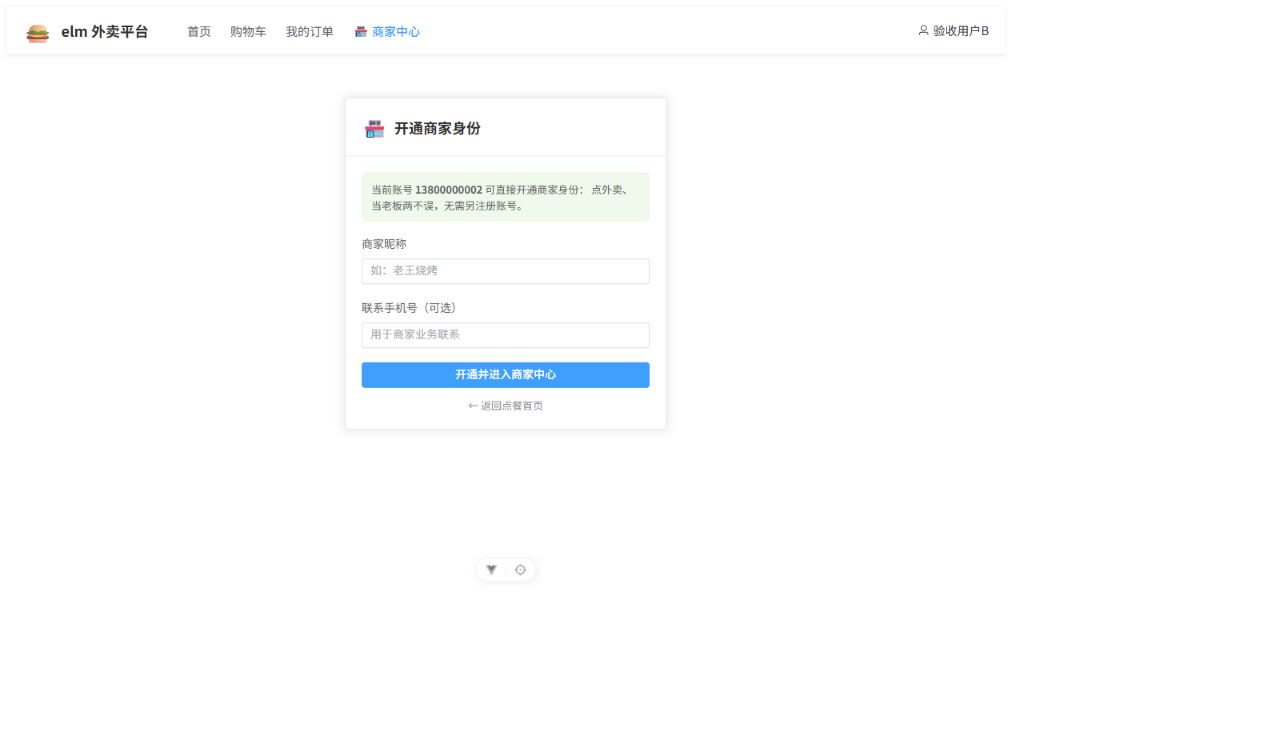
\includegraphics[keepaspectratio,alt={补充的商家身份入口}]{figures/cross/2026-9-16-sep-elm-SRS对照验收-商家入口.png}}

\textbf{结论}：已实现并通过。统一 Account、User 与 Merchant 的主流程符合
SRS

\textbf{本轮未测试项}：重复开通商家身份、联系电话边界和其他商家资源权限，本轮主要确认已有账号可以追加
Merchant 身份

\subsection{FR-MERCHANT-02
商家经营状态}\label{fr-merchant-02-ux5546ux5bb6ux7ecfux8425ux72b6ux6001}

\textbf{需求目标}：Merchant 支持 OPERATING 和
TEMP\_CLOSED，临时闭店时旗下店铺对外不可营业，恢复后店铺自身状态继续生效

\textbf{实际验收}：商家 C 将店铺设置为``临时休息''，用户 A
刷新首页后看到``休息中''，恢复后重新显示``营业中''

\pandocbounded{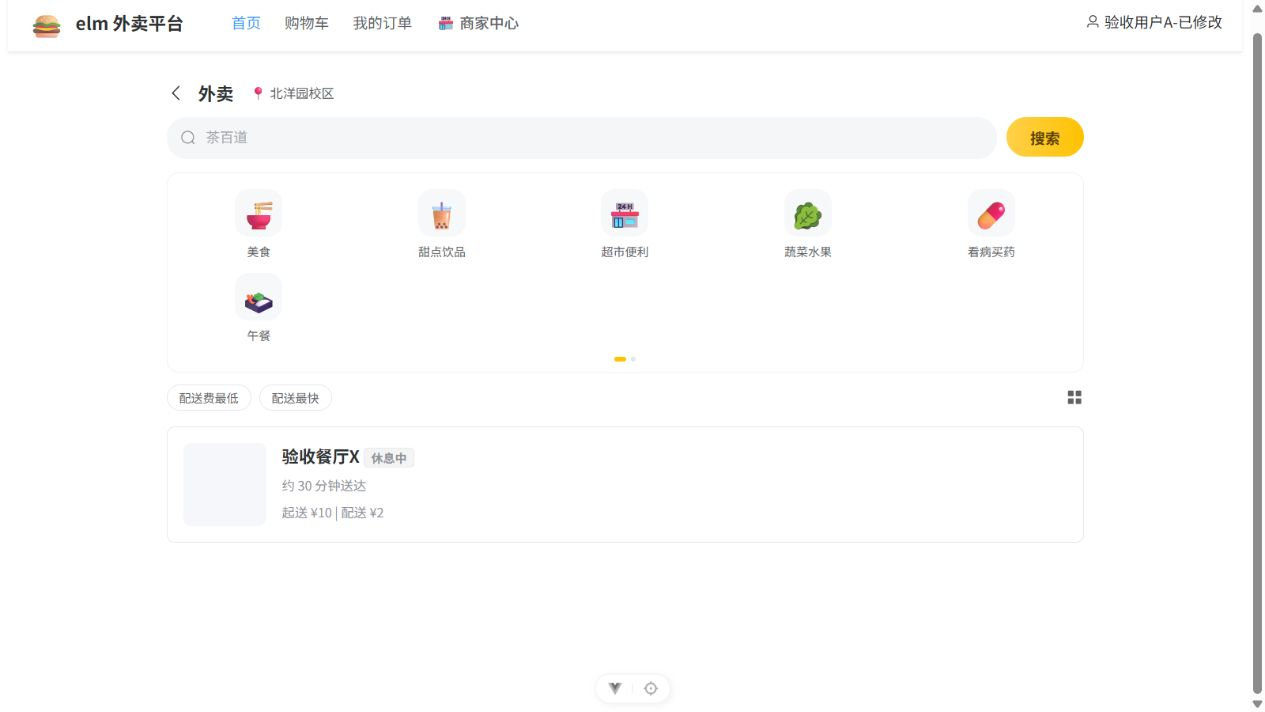
\includegraphics[keepaspectratio,alt={店铺休息状态证据}]{figures/cross/2026-9-16-sep-elm-SRS验收截图-消费者侧休息状态.png}}

\textbf{结论}：已实现并通过页面同步验证

\textbf{改进建议}：补测 Merchant 总状态与 Store
自身状态叠加时的组合结果，确认不会错误修改 Store
原始状态；自动营业时间不属于当前范围，不应作为缺陷

\subsection{FR-STORE-01
创建店铺}\label{fr-store-01-ux521bux5efaux5e97ux94fa}

\textbf{需求目标}：一个 Merchant 可以创建多个 Store，关系为 Merchant 1:N
Store

\textbf{实际验收}：商家 C 创建了店铺 X 和店铺
Y，两个店铺均能够在商家侧展示

\pandocbounded{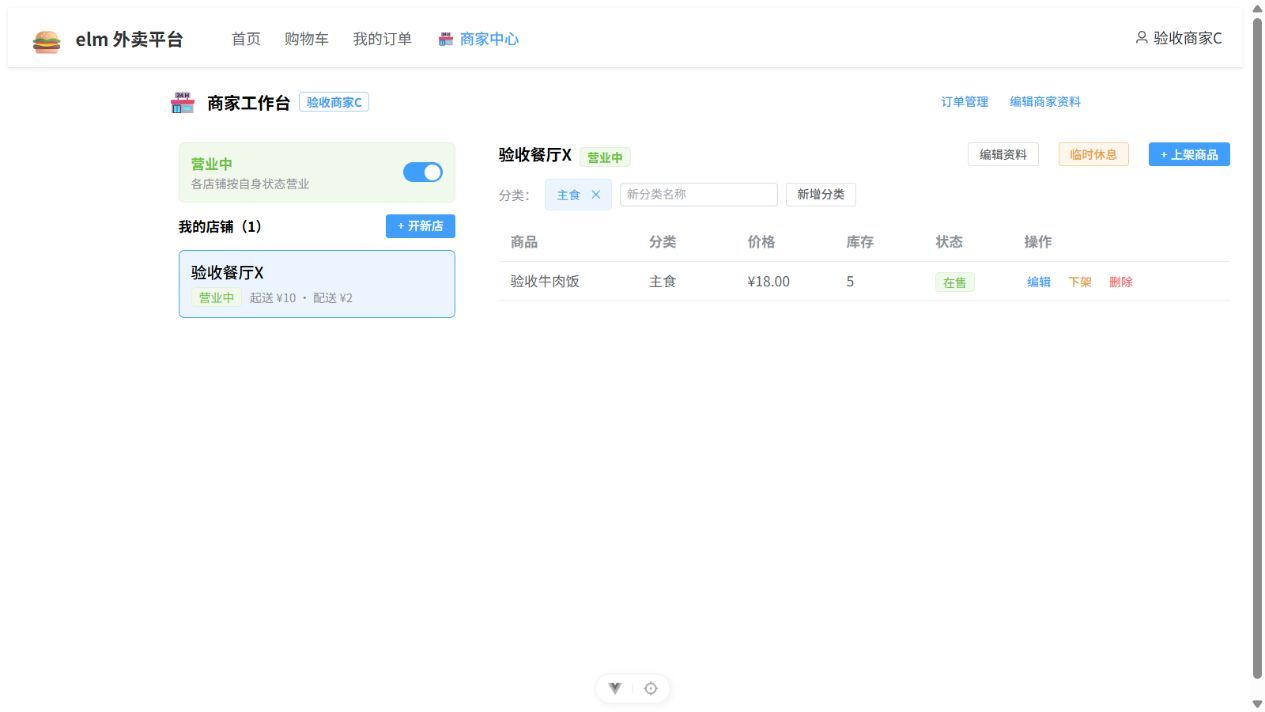
\includegraphics[keepaspectratio,alt={店铺创建证据}]{figures/cross/2026-9-16-sep-elm-SRS验收截图-06-商家工作台.png}}

\textbf{结论}：已实现并通过多店铺主流程验证

\textbf{本轮未测试项}：店铺名称重复、异常费用、异常配送时间和复杂权限边界，本轮主要确认商家可以创建多个店铺并展示基础资料

\subsection{FR-STORE-02
店铺列表}\label{fr-store-02-ux5e97ux94faux5217ux8868}

\textbf{需求目标}：用户查询可展示店铺，至少显示名称、图片、营业状态、配送费、起送金额和预计配送时间

\textbf{实际验收}：用户 A
首页显示真实店铺、营业状态、配送费、起送金额和配送时间

\pandocbounded{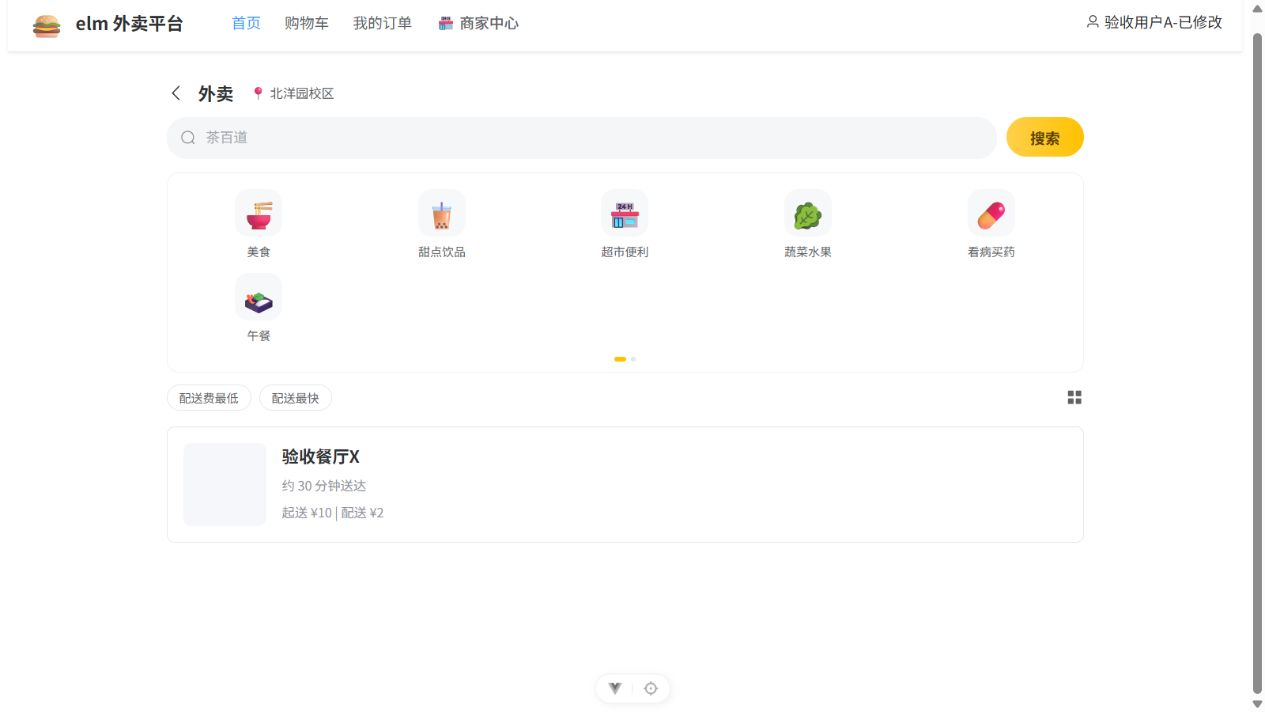
\includegraphics[keepaspectratio,alt={店铺列表证据}]{figures/cross/2026-9-16-sep-elm-SRS验收截图-01-用户首页.png}}

\pandocbounded{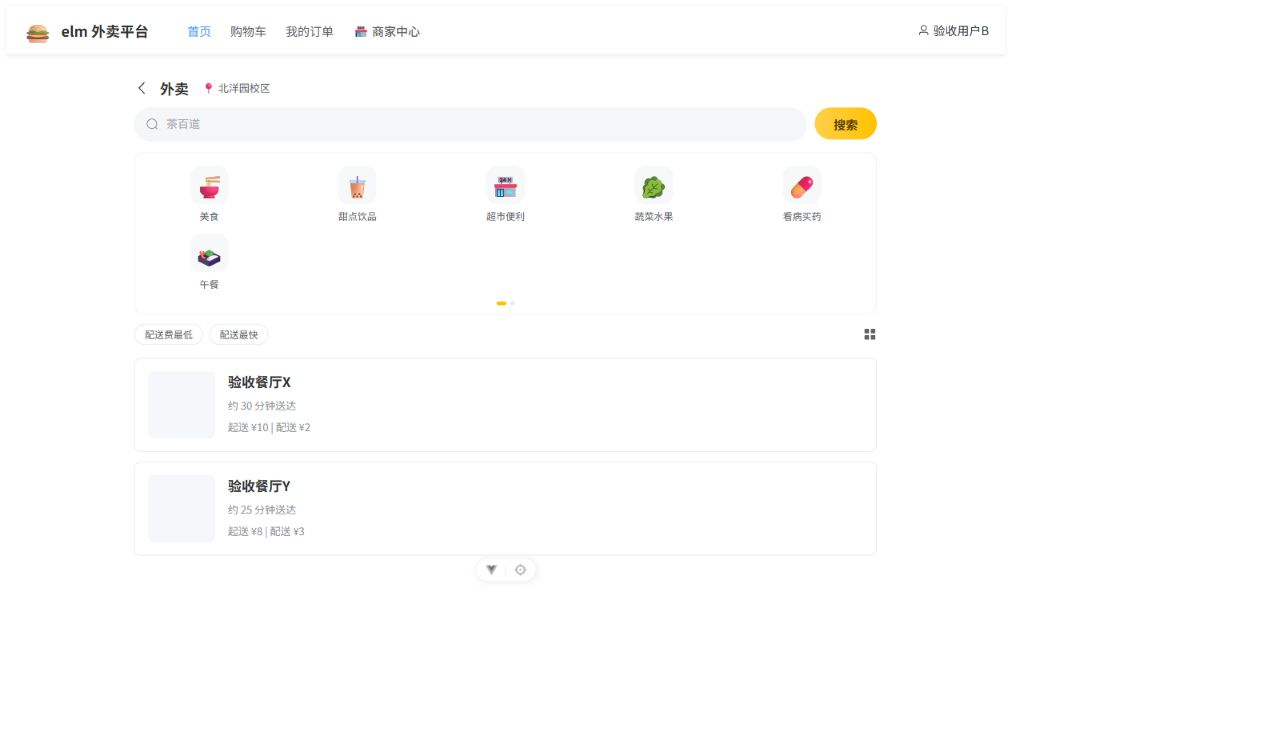
\includegraphics[keepaspectratio,alt={补充的首页店铺列表}]{figures/cross/2026-9-16-sep-elm-SRS对照验收-首页店铺列表.png}}

\textbf{结论}：已实现并通过

\textbf{改进建议}：确认无图片、店铺休息、店铺为空和多个店铺排序时页面是否有稳定的空状态与错误状态

\subsection{FR-STORE-03
店铺详情}\label{fr-store-03-ux5e97ux94faux8be6ux60c5}

\textbf{需求目标}：用户可以查询单个店铺的详细信息，并查看该店铺商品与分类

\textbf{实际验收}：用户 A
进入店铺详情，可以看到公告、营业状态、配送信息、分类和商品

\pandocbounded{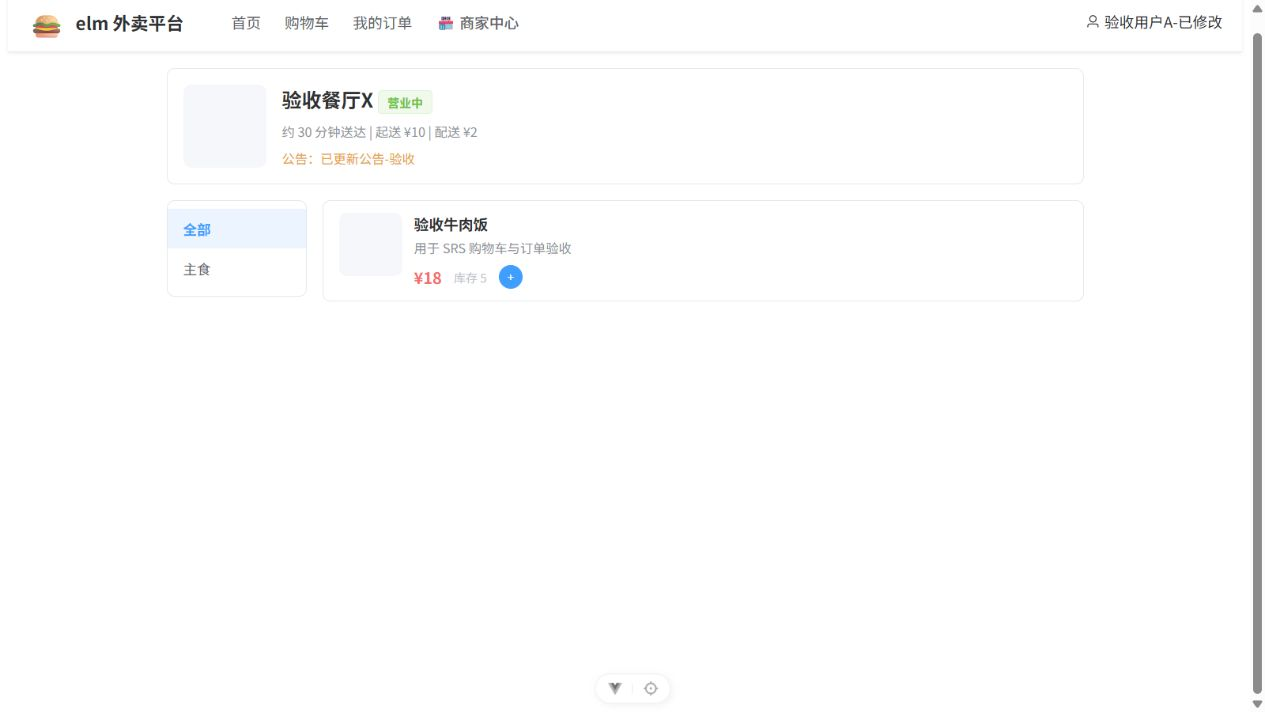
\includegraphics[keepaspectratio,alt={店铺详情证据}]{figures/cross/2026-9-16-sep-elm-SRS验收截图-02-店铺商品.png}}

\pandocbounded{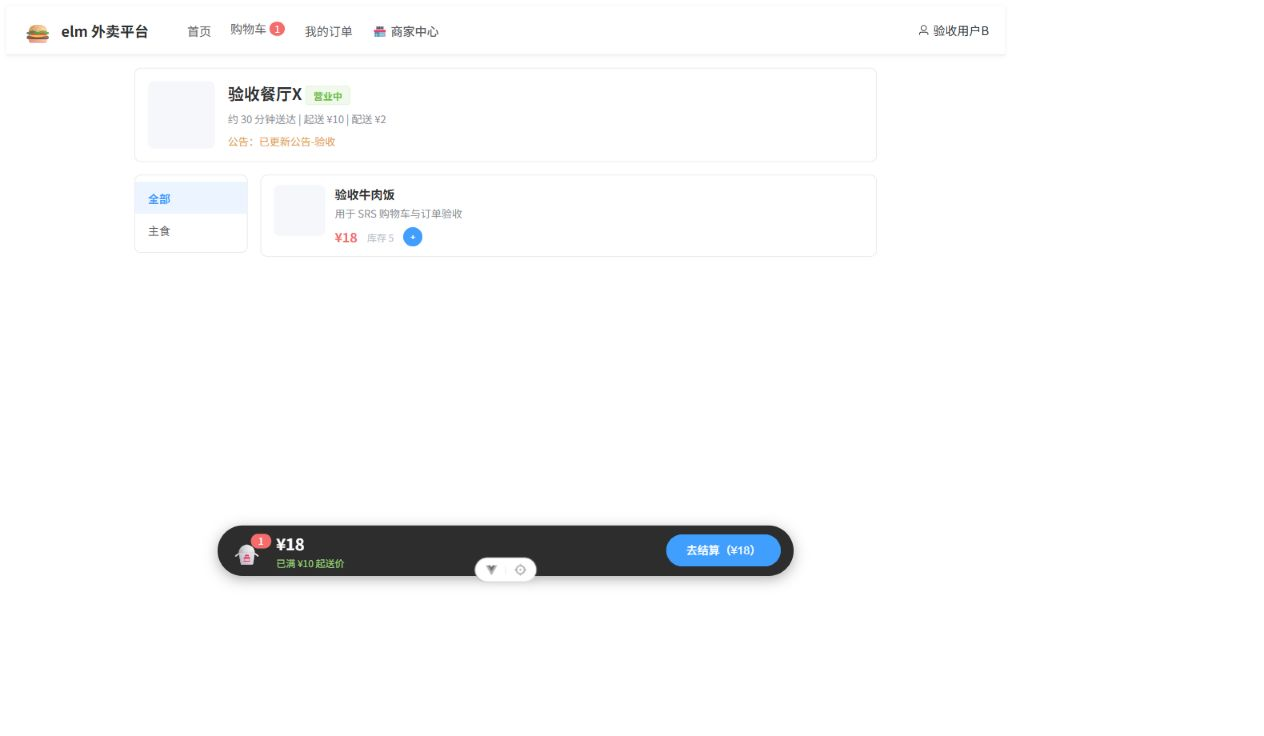
\includegraphics[keepaspectratio,alt={补充的店铺详情页面}]{figures/cross/2026-9-16-sep-elm-SRS对照验收-店铺详情.png}}

\textbf{结论}：已实现并通过页面验证

\subsection{FR-STORE-04
店铺营业状态}\label{fr-store-04-ux5e97ux94faux8425ux4e1aux72b6ux6001}

\textbf{需求目标}：Store 拥有自己的营业状态，Merchant 总状态和 Store
状态共同决定对外营业状态，当前不实现自动营业时间调度

\textbf{实际验收}：商家切换休息状态后消费者侧同步显示，恢复后状态恢复正常

\textbf{结论}：已实现当前人工切换范围，自动时间调度不属于本轮缺陷

\subsection{FR-STORE-05
店铺资料维护}\label{fr-store-05-ux5e97ux94faux8d44ux6599ux7ef4ux62a4}

\textbf{需求目标}：商家只能维护自己店铺的名称、公告、配送费、起送价和预计配送时间，支持部分更新，并拒绝空名称、负数费用和其他商家的店铺

\textbf{实际验收}：商家 C 只修改公告，页面提示更新成功，其他字段保持原值

\pandocbounded{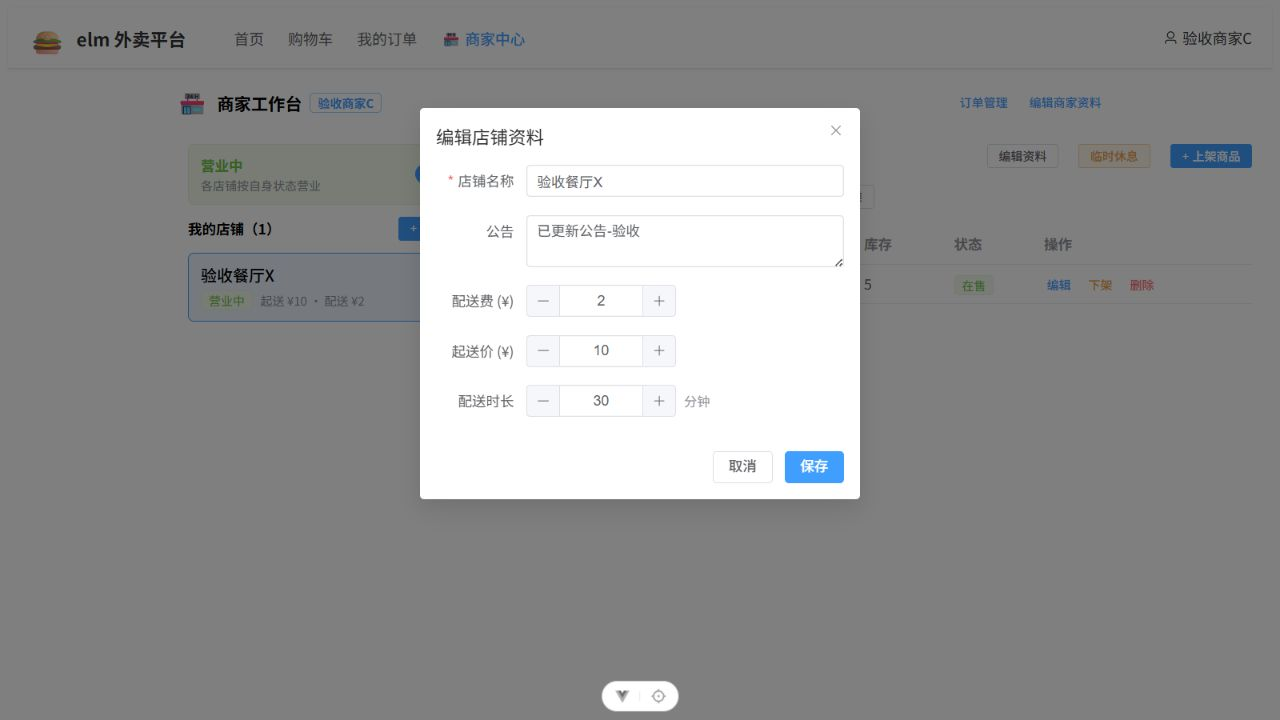
\includegraphics[keepaspectratio,alt={店铺资料更新证据}]{figures/cross/2026-9-16-sep-elm-SRS验收截图-店铺资料更新.png}}

\textbf{结论}：部分通过。部分更新已验证，空名称、负数费用和其他商家店铺等异常操作本轮未测试

\textbf{改进建议}：增加字段级参数和归属权限测试，并检查客户端是否可能自行提交其他
storeId

\subsection{FR-CATEGORY-01
商品分类}\label{fr-category-01-ux5546ux54c1ux5206ux7c7b}

\textbf{需求目标}：每个 Store 可以拥有多个 Category，每个 Product
只属于一个 Category

\textbf{实际验收}：商家 C
创建``主食''和``饮品''分类，商品分别归属对应分类，消费者侧按分类展示

\textbf{结论}：已实现并通过基础关系验证

\subsection{FR-PRODUCT-01
商品管理}\label{fr-product-01-ux5546ux54c1ux7ba1ux7406}

\textbf{需求目标}：商家管理自己店铺商品，商品包含名称、描述、图片、价格、库存、状态、Store
和 Category

\textbf{实际验收}：商家创建``验收牛肉饭''和``验收奶茶''，页面显示价格、库存、分类和在售状态

\pandocbounded{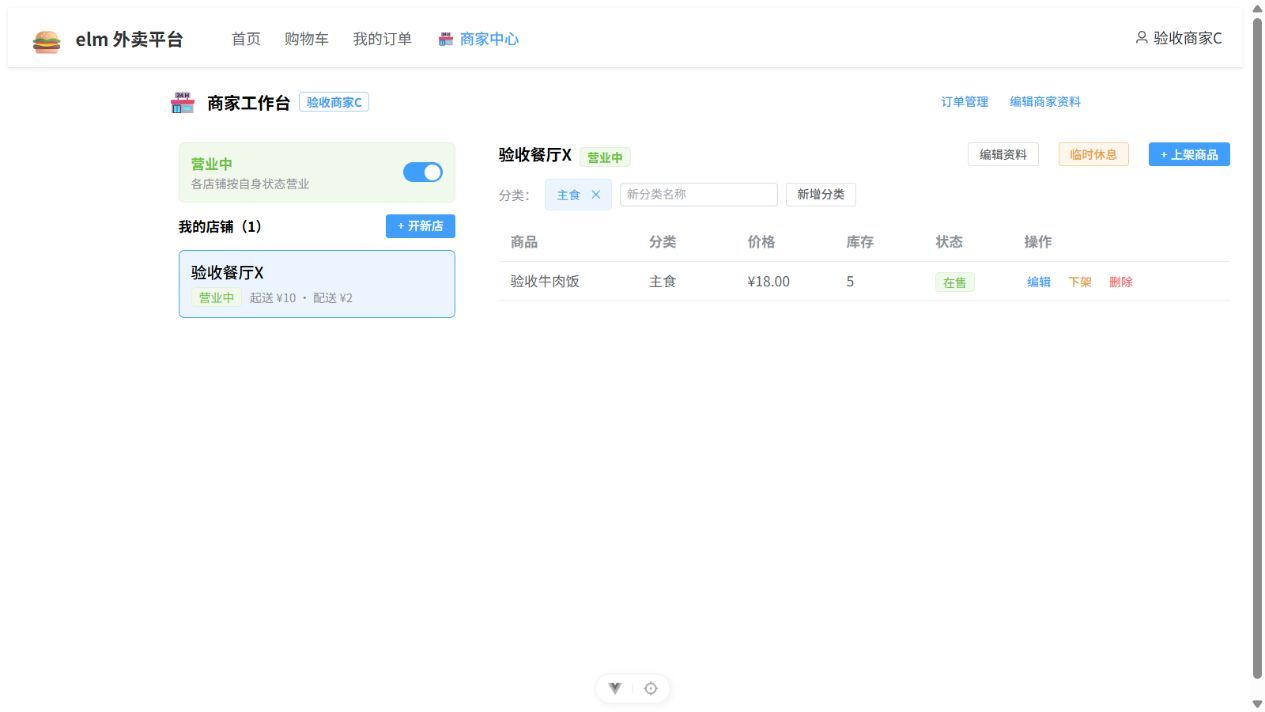
\includegraphics[keepaspectratio,alt={商品管理证据}]{figures/cross/2026-9-16-sep-elm-SRS验收截图-06-商家工作台.png}}

\textbf{结论}：基础商品创建、分类归属、价格、库存和状态已实现；描述和图片的完整展示、异常价格、负库存及其他商家商品权限本轮未测试

\subsection{FR-PRODUCT-02 / FR-PRODUCT-03
商品列表与详情}\label{fr-product-02--fr-product-03-ux5546ux54c1ux5217ux8868ux4e0eux8be6ux60c5}

\textbf{需求目标}：用户可以按店铺查询商品列表并查看单个商品详情

\textbf{实际验收}：用户 A 进入店铺详情后看到店铺 X 和 Y
的商品，能够查看商品名称、价格和库存相关展示

\textbf{结论}：已实现并通过基础页面验证，异常商品
ID、下架商品详情和不存在商品的 404 本轮未测试

\subsection{FR-PRODUCT-04
商品库存}\label{fr-product-04-ux5546ux54c1ux5e93ux5b58}

\textbf{需求目标}：加购不扣库存，下单时校验状态和库存，成功扣减，失败不产生不完整订单

\textbf{实际验收}：加购和修改数量后，商家页面未观察到库存立即减少；超库存数量输入后页面回退到
1，没有保留非法数量

\textbf{结论}：部分通过。页面初步符合不预占库存，但下单扣减、库存不足下单失败和取消恢复本轮未做数据层核对

\textbf{改进建议}：用库存为 1
和库存接近上限的商品测试下单成功、下单失败、取消订单、重复取消和并发下单，并记录
Product.stock、Order、OrderItem 和 CartItem 的变化

\section{购物车需求对照}\label{4-ux8d2dux7269ux8f66ux9700ux6c42ux5bf9ux7167}

\subsection{FR-CART-01
加入购物车}\label{fr-cart-01-ux52a0ux5165ux8d2dux7269ux8f66}

\textbf{需求目标}：请求只提交 productId 和 quantity，由当前 Token 推导
User 和 Product 所属 Store，同一 user + store + product
不建立重复行，再次加入应累加数量

\textbf{实际验收}：用户 A 加入店铺 X 和 Y
的商品，商品能够进入购物车；同一商品数量可以继续调整

\pandocbounded{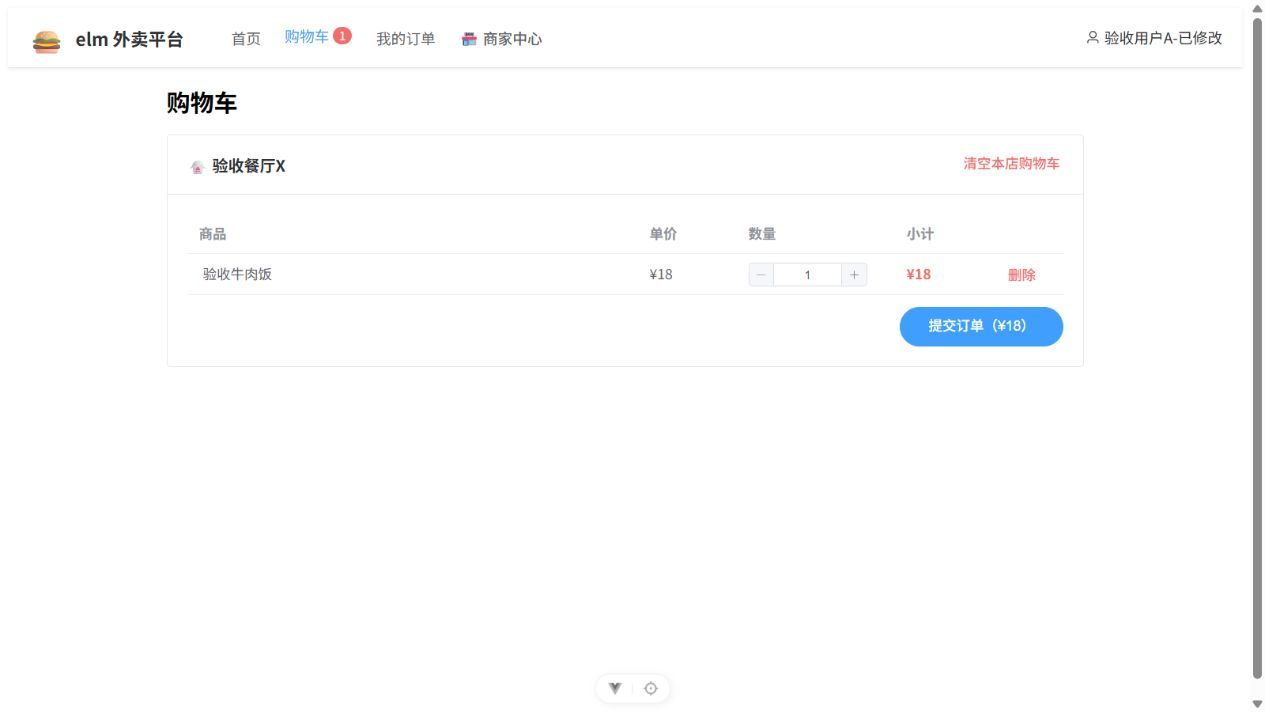
\includegraphics[keepaspectratio,alt={购物车证据}]{figures/cross/2026-9-16-sep-elm-SRS验收截图-03-购物车.png}}

\textbf{结论}：基础加入功能通过，但重复加入、库存不足、商品下架和
stock\textless=0 等异常场景本轮未测试

\textbf{改进建议}：重复点击加入同一商品，检查数据库唯一约束和数量累加结果，并确认失败时原
CartItem 数量不改变

\subsection{FR-CART-02
修改数量}\label{fr-cart-02-ux4feeux6539ux6570ux91cf}

\textbf{需求目标}：quantity 是新的绝对数量，必须 \textgreater=1
且不得超过当前库存，条目只能属于当前 User，失败不得破坏原数量

\textbf{实际验收}：用户 A 将商品数量从 1 调整为
2，页面能够重新计算小计；输入超过库存的 7 后数量回退到 1

\pandocbounded{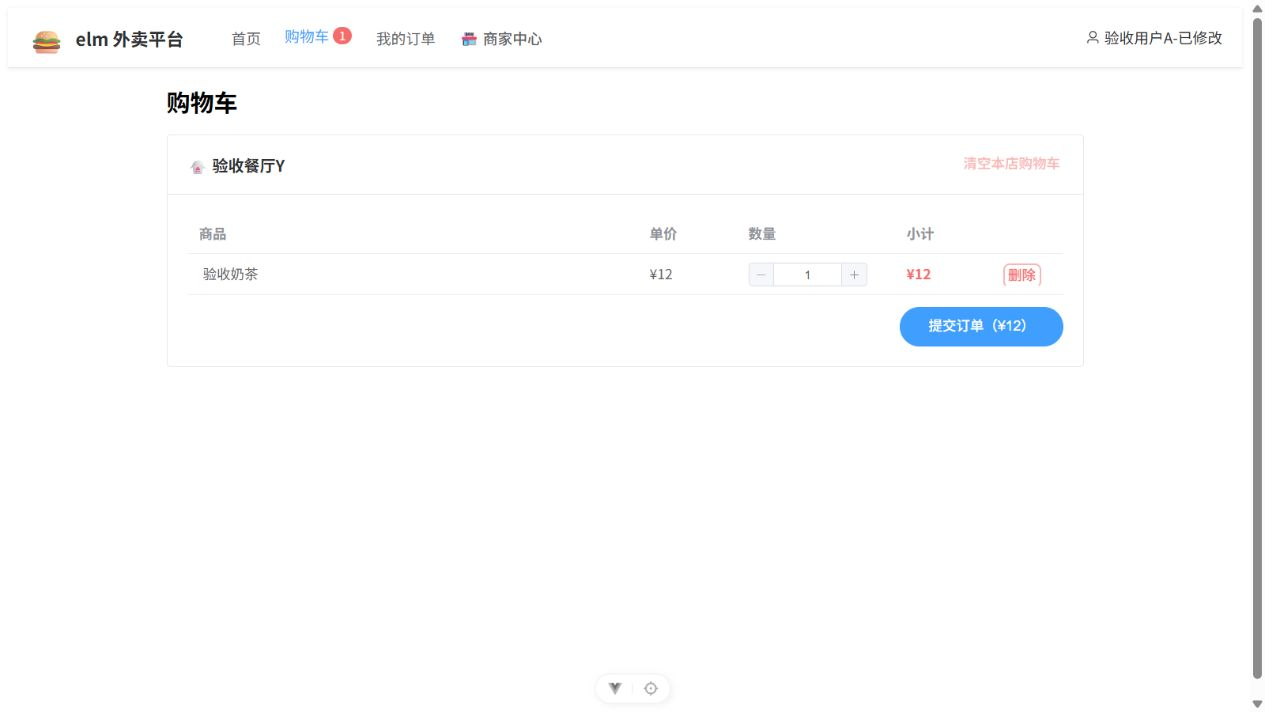
\includegraphics[keepaspectratio,alt={超库存边界证据}]{figures/cross/2026-9-16-sep-elm-SRS验收截图-超库存边界.png}}

\textbf{结论}：正常修改通过，超库存数据未保留，但页面缺少明确``库存不足''反馈，接口
400 尚未确认

\subsection{FR-CART-03
删除购物车商品}\label{fr-cart-03-ux5220ux9664ux8d2dux7269ux8f66ux5546ux54c1}

\textbf{需求目标}：只能删除当前 User 的 CartItem，删除为物理
DELETE，其他用户条目统一 404

\textbf{实际验收}：本轮通过店铺清空流程间接验证了购物车条目删除，店铺 X
清空后条目从页面消失

\textbf{结论}：页面行为通过，单条删除、他人 itemId 和已删除 itemId
等异常场景本轮未测试

\subsection{FR-CART-04
查询购物车}\label{fr-cart-04-ux67e5ux8be2ux8d2dux7269ux8f66}

\textbf{需求目标}：查询当前用户全部购物车，按 User + Store
隔离，允许同时保留多个店铺购物车，返回商品和店铺展示信息

\textbf{实际验收}：用户 A 同时加入 X、Y
两家店铺商品，购物车出现两个店铺区块；用户 B 登录后购物车为空

\pandocbounded{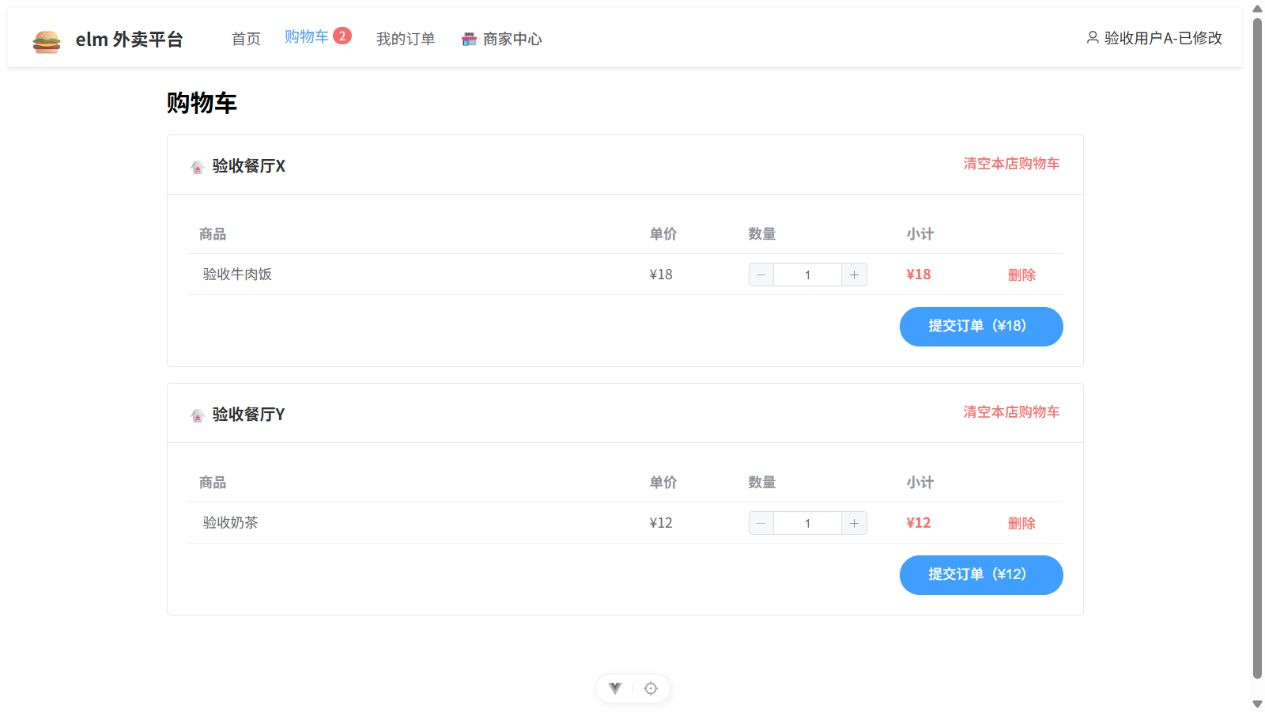
\includegraphics[keepaspectratio,alt={跨店购物车证据}]{figures/cross/2026-9-16-sep-elm-SRS验收截图-跨店购物车.png}}

\pandocbounded{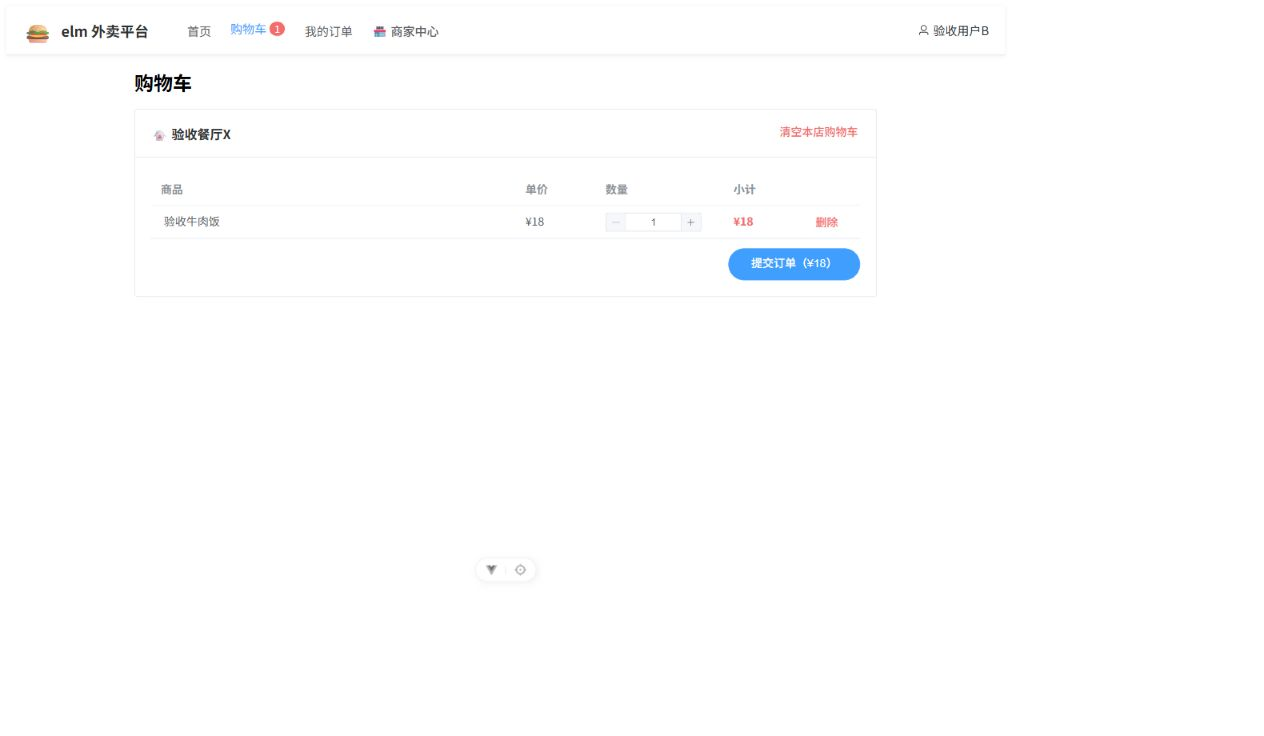
\includegraphics[keepaspectratio,alt={补充的购物车状态}]{figures/cross/2026-9-16-sep-elm-SRS对照验收-购物车状态.png}}

\pandocbounded{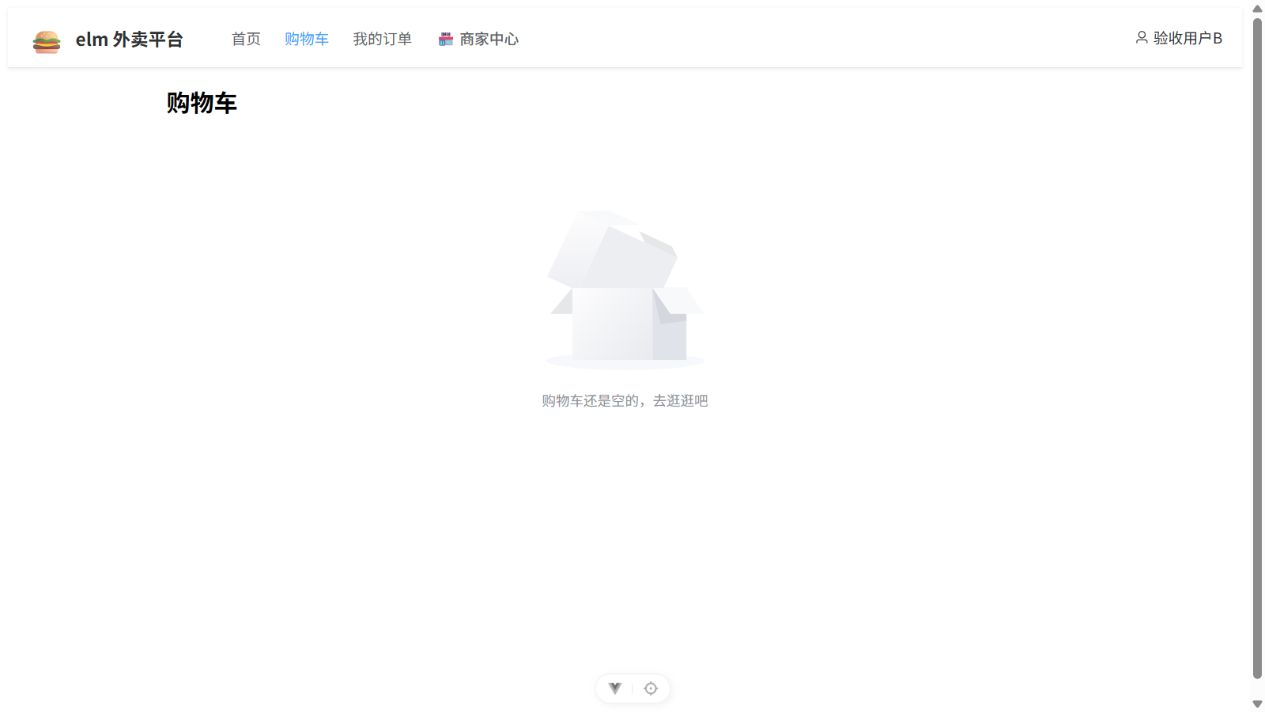
\includegraphics[keepaspectratio,alt={用户 B 隔离证据}]{figures/cross/2026-9-16-sep-elm-SRS验收截图-用户B购物车隔离.png}}

\textbf{结论}：已实现并通过跨店和跨用户页面隔离验证

\subsection{FR-CART-05
购物车与库存}\label{fr-cart-05-ux8d2dux7269ux8f66ux4e0eux5e93ux5b58}

\textbf{需求目标}：加购、改数量、删除和清空购物车都不得修改
Product.stock，不实现库存预占和超时释放

\textbf{实际验收}：加购及改数量后商家侧未观察到库存即时减少

\textbf{结论}：初步通过，仍需数据库精确值和并发行为证据；库存预占、库存锁和超时释放不属于当前范围

\subsection{FR-CART-06
清空购物车}\label{fr-cart-06-ux6e05ux7a7aux8d2dux7269ux8f66}

\textbf{需求目标}：不带 shopId 清空当前用户全部条目，带 shopId
只清空当前店铺，不能影响其他用户，清空不修改库存

\textbf{实际验收}：清空店铺 X 后店铺 Y 仍保留

\pandocbounded{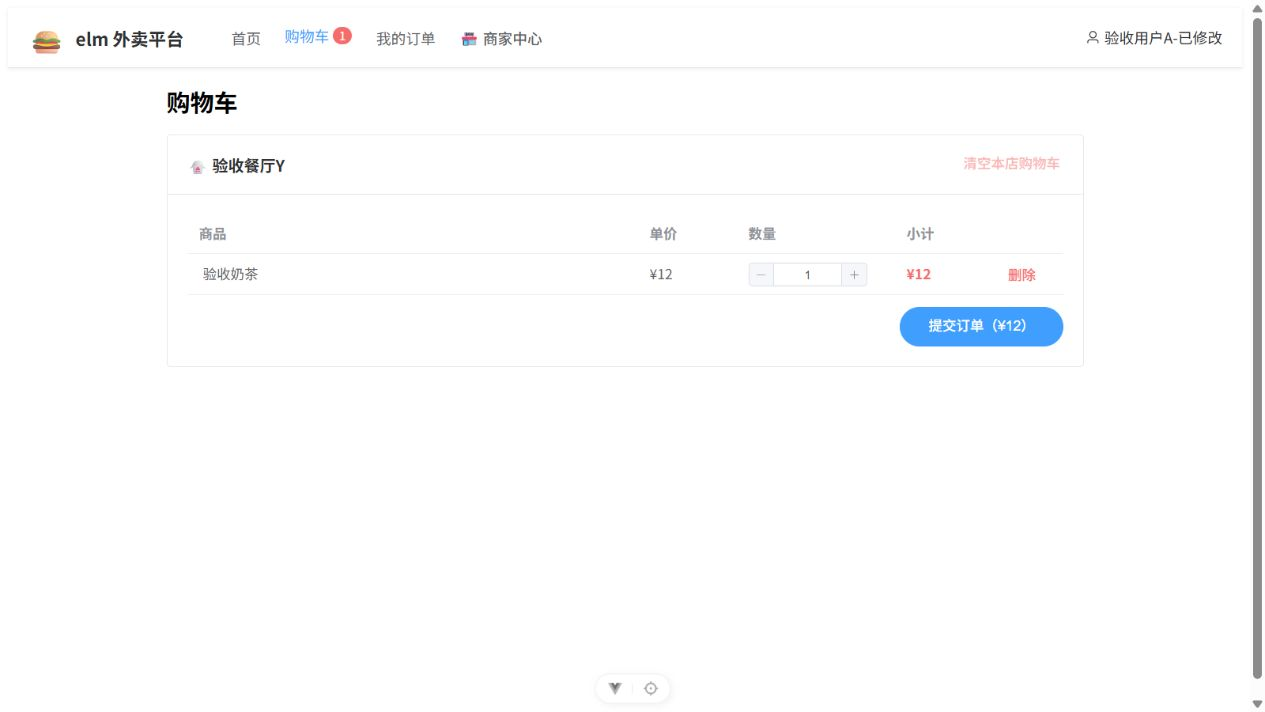
\includegraphics[keepaspectratio,alt={指定店铺清空证据}]{figures/cross/2026-9-16-sep-elm-SRS验收截图-指定店铺清空.png}}

\textbf{结论}：带店铺条件清空通过，不带 shopId
的全量清空、空购物车重复清空和失败时数据保留本轮未测试

\section{订单需求对照}\label{5-ux8ba2ux5355ux9700ux6c42ux5bf9ux7167}

\subsection{FR-ORDER-01
创建订单}\label{fr-order-01-ux521bux5efaux8ba2ux5355}

\textbf{需求目标}：一次订单只处理一个 Store，校验商品状态和库存，创建
Order 与 OrderItem，扣减库存，清空本店购物车，并保证失败整体事务回滚

\textbf{实际验收}：用户 A
从购物车提交订单，填写地址和备注，订单详情显示店铺、商品、单价、数量、小计、总金额、地址和备注

\pandocbounded{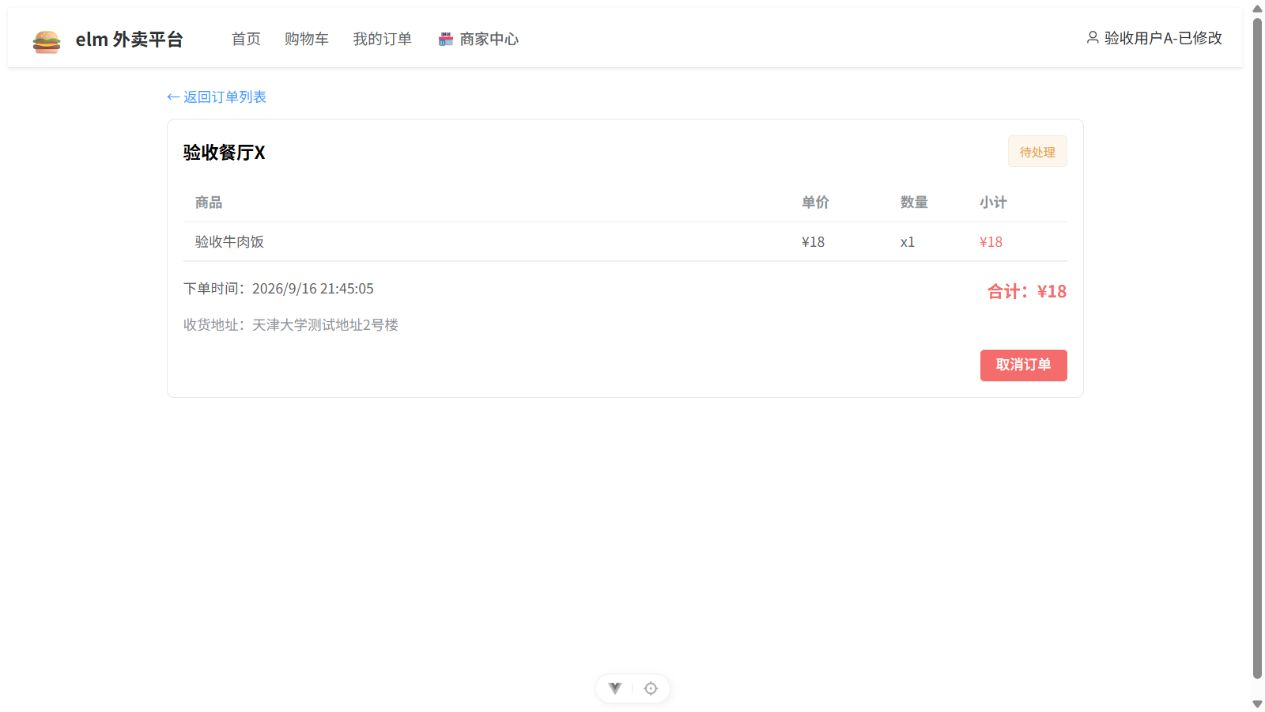
\includegraphics[keepaspectratio,alt={新订单详情证据}]{figures/cross/2026-9-16-sep-elm-SRS验收截图-04-新订单详情.png}}

\textbf{结论}：正常订单创建通过，跨店订单禁止、库存不足失败和创建失败后的订单、购物车、库存回滚本轮未测试

\textbf{改进建议}：先在购物车保留两个店铺商品，再只结算一个店铺，确认另一店铺购物车保留；构造库存不足和商品下架场景，检查失败后订单、库存和购物车是否保持一致；连续点击提交和提交后刷新，检查是否产生重复订单

\subsection{FR-ORDER-02 OrderItem
商品快照}\label{fr-order-02-orderitem-ux5546ux54c1ux5febux7167}

\textbf{需求目标}：OrderItem 保存
product\_id、product\_name、price、quantity，商品后续改名或改价不得影响历史订单

\textbf{实际验收}：订单详情能够展示下单时的商品名称、单价、数量和小计

\textbf{结论}：页面初步通过，但尚未执行下单后修改商品名称和价格再回看历史订单的反向验证

\textbf{改进建议}：增加商品主数据变更前后对比截图，并从数据库确认
OrderItem 快照字段独立保存

\subsection{FR-ORDER-03
配送地址}\label{fr-order-03-ux914dux9001ux5730ux5740}

\textbf{需求目标}：Order 直接保存本次配送地址快照，不建设 UserAddress
地址簿

\textbf{实际验收}：测试地址``天津大学测试地址1号楼''成功保存并在订单详情展示

\textbf{结论}：已实现并通过，地址簿、多地址 CRUD 等明确不属于当前范围

\subsection{FR-ORDER-04
订单状态}\label{fr-order-04-ux8ba2ux5355ux72b6ux6001}

\textbf{需求目标}：当前仅支持 CREATED 和
CANCELLED，不实现支付、配送、骑手和复杂状态机

\textbf{实际验收}：订单创建后显示待处理，取消后显示已取消，取消按钮消失

\pandocbounded{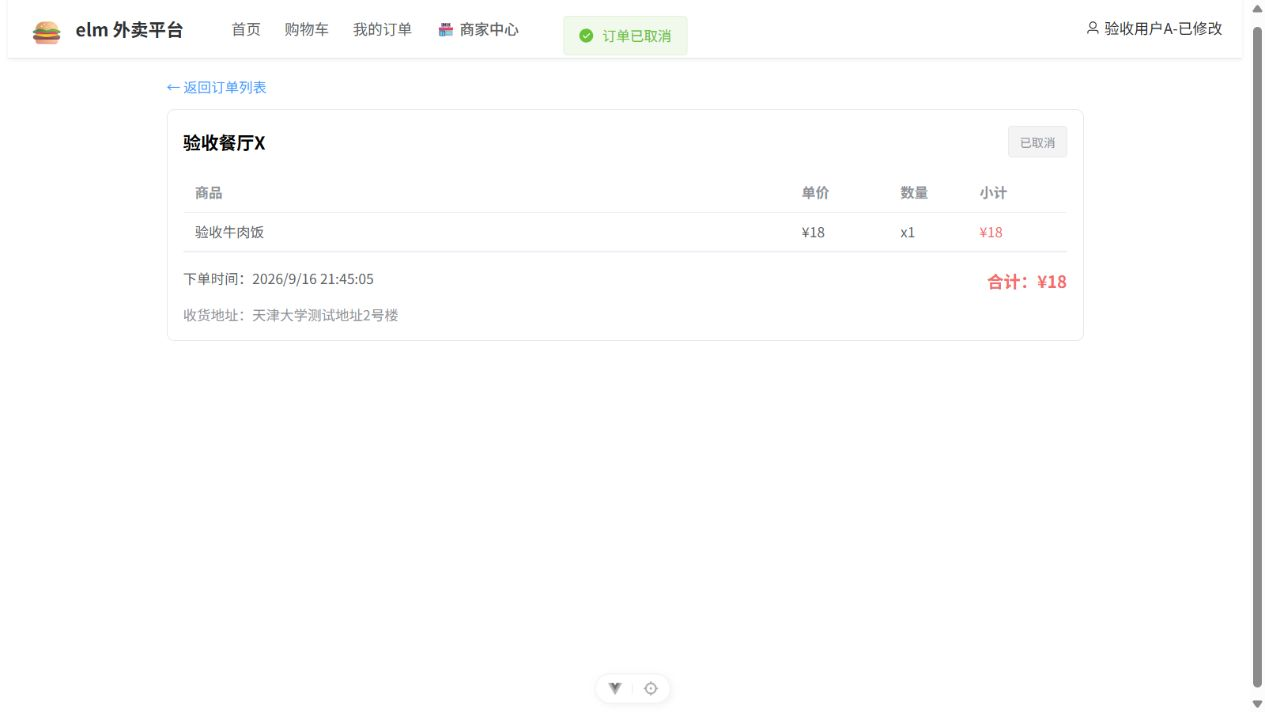
\includegraphics[keepaspectratio,alt={取消订单证据}]{figures/cross/2026-9-16-sep-elm-SRS验收截图-05-取消订单.png}}

\textbf{结论}：当前状态主流程通过，重复取消、非法状态转换和接口状态码本轮未测试；支付、退款、配送等不属于缺陷范围

\subsection{FR-ORDER-05
查询订单}\label{fr-order-05-ux67e5ux8be2ux8ba2ux5355}

\textbf{需求目标}：用户查询自己的订单列表、详情和当前状态，不存在订单返回
404

\textbf{实际验收}：用户 A 可以查看订单详情和列表，用户 B 看不到用户 A
的订单

\pandocbounded{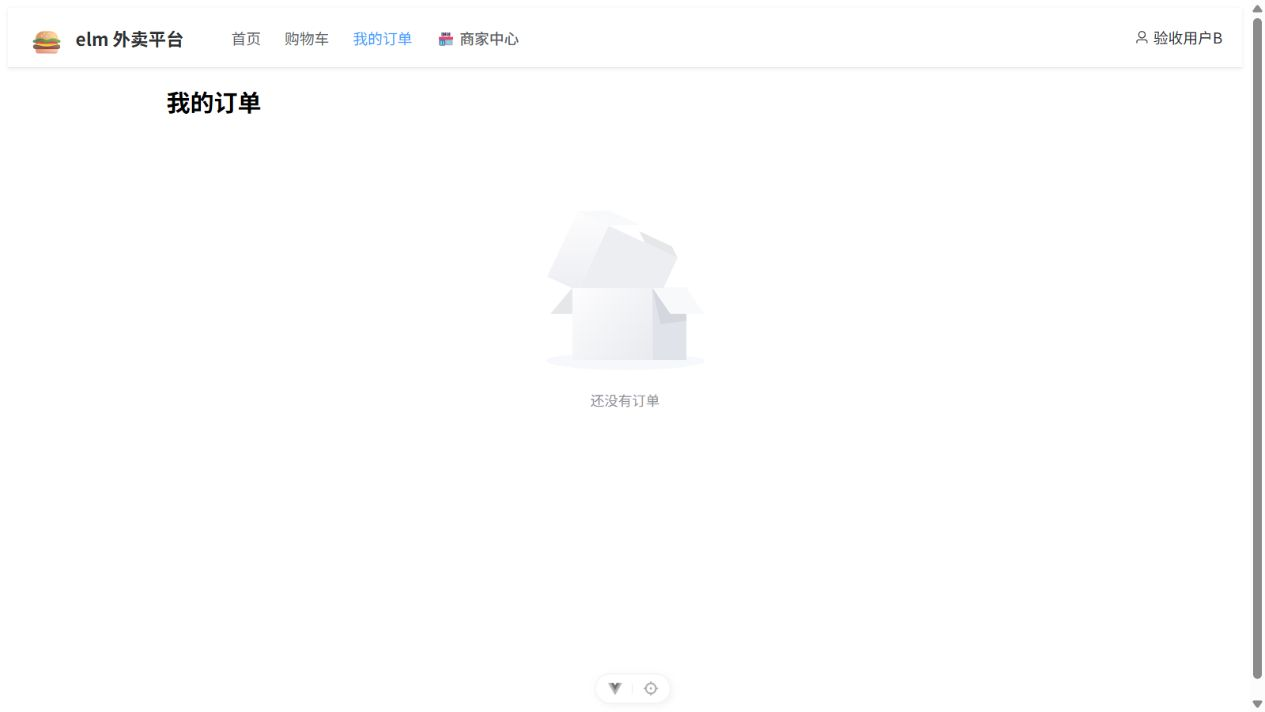
\includegraphics[keepaspectratio,alt={用户 B 订单隔离证据}]{figures/cross/2026-9-16-sep-elm-SRS验收截图-用户B订单隔离.png}}

\pandocbounded{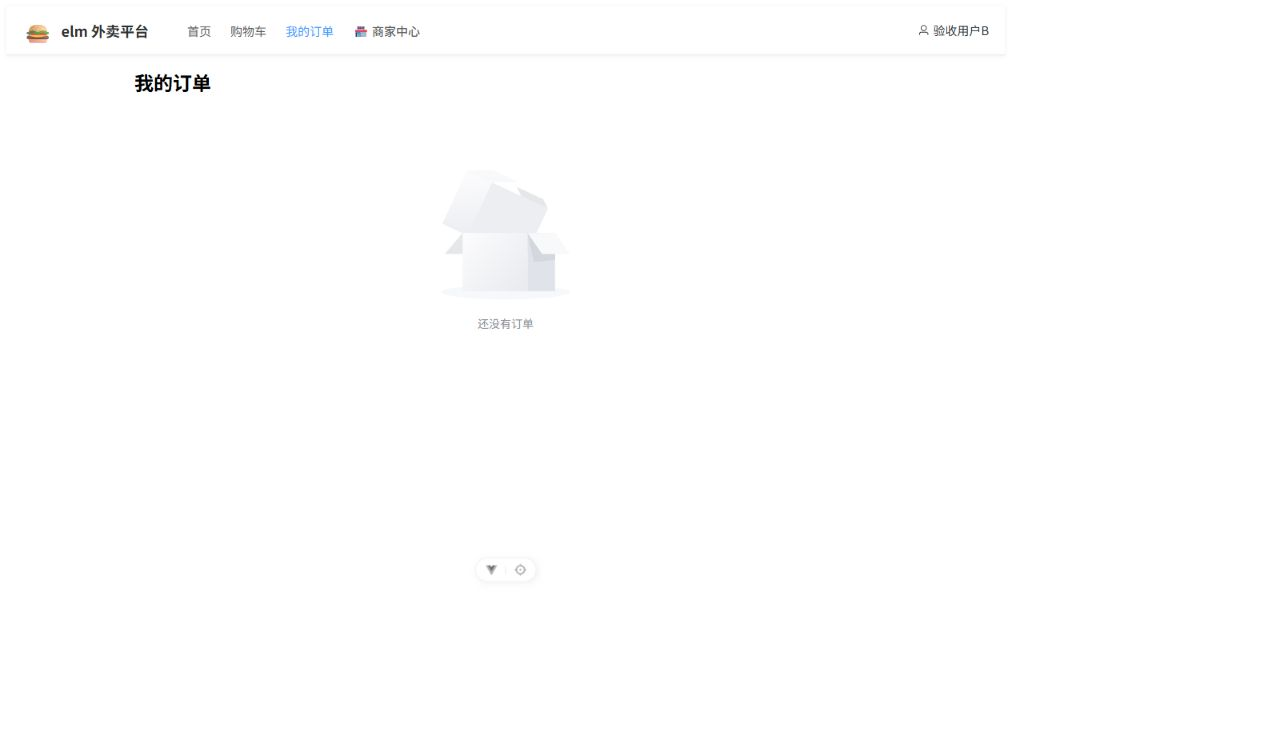
\includegraphics[keepaspectratio,alt={补充的订单列表页面}]{figures/cross/2026-9-16-sep-elm-SRS对照验收-订单列表.png}}

\textbf{结论}：正常查询和跨用户页面隔离通过，不存在订单、他人 orderId
和未登录访问本轮未测试

\subsection{FR-ORDER-06
取消订单}\label{fr-order-06-ux53d6ux6d88ux8ba2ux5355}

\textbf{需求目标}：仅允许用户取消自己的 CREATED
订单，取消与库存恢复在同一事务内，CANCELLED 不得重复取消

\textbf{实际验收}：用户 A
取消自己的待处理订单后状态变为``已取消''，按钮消失

\textbf{结论}：取消状态变化通过，库存恢复精确值、重复取消、他人订单和事务一致性本轮未测试

\textbf{改进建议}：对比下单前、下单后和取消后的
Product.stock，重复执行取消并检查库存是否被重复增加，同时使用另一账号尝试取消该订单

\subsection{FR-ORDER-07
商户侧只读订单}\label{fr-order-07-ux5546ux6237ux4fa7ux53eaux8bfbux8ba2ux5355}

\textbf{需求目标}：Merchant 只能查看自己旗下 Store
的订单列表和详情，身份由 Token 推导，不接受前端 merchantId 或 storeId
作为身份依据，接口只读

\textbf{实际验收}：商家 C
能查看自己店铺订单列表和订单详情，包括买家、金额、地址、状态和商品快照，页面没有订单修改或履约操作

\pandocbounded{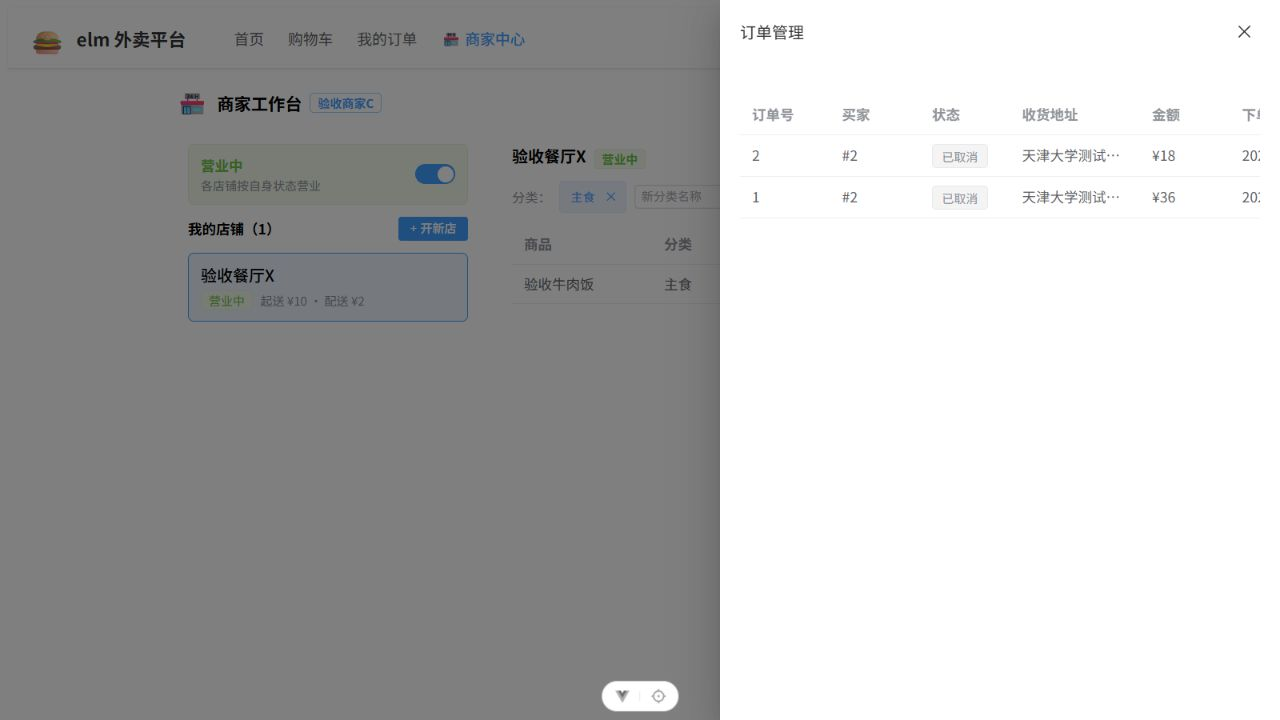
\includegraphics[keepaspectratio,alt={商家订单列表证据}]{figures/cross/2026-9-16-sep-elm-SRS验收截图-07-商家订单.png}}

\pandocbounded{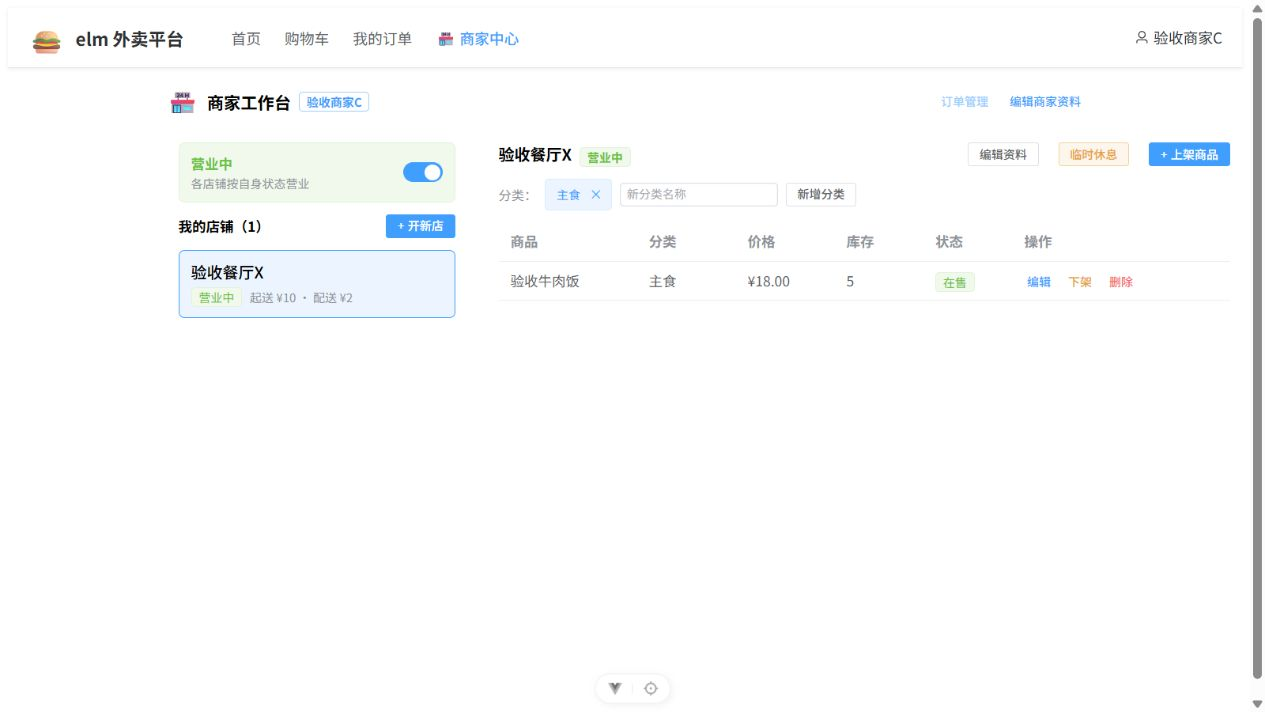
\includegraphics[keepaspectratio,alt={商家订单详情证据}]{figures/cross/2026-9-16-sep-elm-SRS验收截图-商家订单详情.png}}

\textbf{结论}：商家只读查看主流程通过，其他商家订单、伪造
merchantId/storeId、未开通 Merchant 身份和未登录访问本轮未测试

